\documentclass[output=paper]{langscibook}
\author{Bart Karstens \affiliation{Vrije Universiteit Amsterdam}}
\title{The Impact of Russian Formalism on Linguistic Structuralism}
\label{chap:karstens}

\abstract{The aim of this chapter is to clarify the relation between Russian formalism, a movement in literary studies, and structuralism. Because leading structuralists such as Mukarovsky (linguistics) and Lévi-Strauss (anthropology) defined their approach in opposition to formalism, we may have the impression that structuralism and formalism are fundamentally different. However, on closer inspection, it turns out that Mukarovsky and Lévi-Strauss targeted specific articulations of formalism. There is a third major variant, namely systemic formalism, which escapes their criticism and can be shown to have influenced structuralism in its earliest phase. First, Tynjanov and Jakobson worked together and co-authored an important short programmatic paper. Second, the genesis of Prague School structuralism should be considered a merger of elements stemming from a multitude of directions. If we do so, we can see how ideas stemming from systemic formalism fitted in with other constituents of linguistic structuralism, and hence how formalism influenced the latter to a significant degree.}
 
\begin{document}
\maketitle

\section{Introduction} 
\label{sec:karstens:intro}

Since the very beginning of structuralism, its relation to Russian formalism has been a matter of dispute. Leading structuralists, such as Jan Mukarovsky (1891--1975) and Claude Lévi-Strauss (1908--2009), emphasized the differences between formalism and structuralism, and members of the Prague Circle even claimed that formalism was \emph{passé} and in need of replacement, as it was marked too much by its mechanistic heritage. In this chapter, I will review the dismissive attitude of structuralists towards formalism. My conclusion is that this attitude applied to a number of articulations of formalism, but \emph{not} to the so-called \emph{systemic} variant, which itself was formulated in response to problems experienced within the formalist programme. From this it follows that a number of key notions of formalism must be considered as constitutive of the structuralist analysis of linguistic phenomena. In my interpretation these key notions include the application of the function concept, the recognition of the systematic recurrence of forms in language, the perspective on language as a system, as well as a system \emph{within} systems, and the analysis of actual manifestations of language in speech and writing with reference to a deeper, underlying system.

I begin by discussing the reasons proponents of structuralism, such as Mukarovsky and Lévi-Strauss, had for their opposition to formalism. Mukarovsky is interesting because he put forward his critique of formalism during the formative days of structuralism in Prague and, according to Toman, Mukarovsky was the second most important representative of Czech structuralism after Roman Jakobson~(1896--1982) \citep[128]{Toman1995}. Lévi-Strauss carried structuralism into the social sciences. I focus on his infamous 1960 critique of Vladimir Propp~(1895--1970) and his \citeyear{Propp1928} book \emph{Morphology of the Folktale}, which met with a late reception in Europe and the United States. Despite the fact that more than 30 years elapsed, both scholars delivered similar forms of critique on formalism, which gives the impression of a clear-cut and deep rift between formalism and structuralism.  

But it is essential to see that formalism was not a unitary movement at all. Following \citet{Steiner1984}, three main types of formalism can be identified, namely mechanical, organic and systemic formalism.\footnote{These labels are based on Steiner's analytical terms. They were not actor’s categories. Significantly, however, what is identified as systemic formalism was sometimes referred to as ``neo-formalism'' by contemporaries.} This classification probably does not even exhaust all possible varieties of formalism that have existed, but it is very useful for the present purposes. As will be made clear in what follows, Mukarovsky dismissed mechanical formalism while Lévi-Strauss targeted organic formalism. In my view, however, systemic formalism possessed a number of properties that escaped both these attacks. 

The main proponent of systemic formalism was Yuri Tynjanov (1894--1943). Tynjanov co-authored a highly influential programmatic paper with Roman Jakobson, which was published in 1928. The nine theses defended in this paper are often referred to as a key text in the genesis of linguistic structuralism. This document thus forms a clear point of contact between systemic formalism and structuralism.\footnote{In historiography, claims of influence always need to be made concrete either by pointing at references in texts or through an investigation of direct personal relations between historical actors. Still relevant in this respect is \citet{Koerner1989}.} In addition, the work of Ferdinand de Saussure (1857--1913) served as an inspiration to both Tynjanov and Jakobson. It is true that formalism was an approach in literary studies and structuralism mainly applied to linguistics. However, the study of literature and the study of language were seen by Tynjanov and Jakobson as complementary parts of the same endeavour. Indeed, the formalism that inspired Jakobson must be embedded in the broader Russian revolutionary cultural climate of the 1910s which included modernist art and futurism (see \citealt[32--33]{Holenstein1975}; see also \citealt{Karstens2017lonely}). 

It is in this context that scholars claimed a place for literary studies as a new independent science. They wanted to base this new science of literature on a set of facts that had to be established without presuppositions. Formalists were in constant debate amongst themselves on how best to pursue this aim. In doing so, different approaches came about, but what they shared was an eschewal of philosophical and psychological speculation. Instead they started to ``borrow'' models from natural sciences, such as biology and chemistry, and made use of technological metaphors to bolster their research programme. Thus, somewhat paradoxically, autonomy for literary studies was claimed through an alignment with science and technology. 

A similar story applies to linguistics.  Structuralism can be seen as a further step in the realization of Saussure's quest to establish an autonomous science of language, centred around the idea of treating languages as value systems of signs. In my view, the formation of structuralism is best studied as a merger of elements stemming from multiple directions.\footnote{For a hybridization perspective on discipline formation, see \citet{Karstens2012}. For the study of interdisciplinarity in terms of a merger of constitutive elements, see \citet{Graff2015} and \citet{Bod2019}. For a contextual study of Jakobson as part of an age of synthesis, see \citet{Karstens2017lonely}.} The ``merger'' perspective allows us to see how systemic formalism provided constituents of early structuralism. Both formalism and structuralism may not have many adherents anymore; however, the systemic way of thinking continues to exert a strong influence on linguistics to this day. Hence it is important to clarify the historical ties between formalism and structuralism in its earliest phase.

\section{Mukarovsky's definition of structuralism as opposed to formalism}
\label{sec:karstens:mukarovsky}

Born in Pisek, Bohemia in 1891, Jan Mukarovsky was among the founders of the Prague Linguistic Circle in 1926. Mukarovsky developed an approach towards literary analysis in which the concepts of structure and structuralism played a central role.\footnote{What follows in the paragraphs below is by and large based on \citep[22--44]{Galan1985}.} He conceived of a structure as a set of elements, organized in a complex hierarchy in which one element dominated over the other elements. This dominant determined how other elements of the structure functioned. For example, in Charlie Chaplin's 1931 silent film \emph{City Lights}, Mukarovsky identified ``expressive gestures'' as the dominant. Other bodily movements and auditory elements (like music) he interpreted as subordinate to the expressive gestures in the film. A literary work or film could thus be interpreted as a relational structure and the main task of the literary critic was to locate the dominant, and the relationships between the dominant and all other elements occurring in the structure. For Mukarovsky, this form of relationalism was holistic: ``Structure is dynamic, containing both the tendencies of convergence and divergence, and its artistic phenomenon which cannot be taken apart since each of its elements gains value only in relationship to the whole'' (Mukarovsky, quoted in \citealt[30]{Galan1985}). Structure could thus also be defined as a whole ``whose nature is determined by the parts and their reciprocal relationships, and which in turn determines the nature and the relationships of the parts'' (Mukarovsky, quoted in \citealt[35]{Galan1985}).

In an interview given to \emph{Prague Weekly} in 1932, Mukarovsky appears to have used the term structuralism for the first time to refer to the new school of literary criticism.\footnote{The first time structuralism was mentioned in print in relation to the study of language is in \citet{Jakobson1929}. I will give this citation below.} In the interview he explicitly mentioned that this new school should be distinguished from formalism. In a 1934 review of the Czech edition of Viktor Shklovsky's (1893--1984) \emph{Theory of Prose} (original edition 1925), it becomes clear how Mukarovsky viewed the opposition between structuralism and formalism. Mukarovsky gave the formalists credit for their polemical extremism and for their rejection of all extrinsic approaches to art that included all kinds of (contextual) interpretation and psychologizing.\footnote{If one thing united all formalists, it was their rejection of both psychologism and subjectivism in literary studies.} According to Mukarovsky, this unqualified emphasis on content had to provoke a radical antithesis emphasizing the form of literary products. 

This shift to form had, however, gone too far. For example, when in Shklovsky's analysis a change in form directly led to a change in content (such as in a passage in \emph{Theory of Prose} on Cervantes’s \emph{Don Quixote}), this was accidental according to Mukarovsky. Shklovsky's research programme would not normally lead to such an analysis because form and content had to be strictly separated. The example demonstrates, however, that even Shklovsky could not avoid accidental identifications of form with meaning. From such examples Mukarovsky drew the conclusion that a synthesis was required between the intrinsic, formalist approach and the extrinsic, interpretative approach, and Mukarovsky explicitly claimed that structuralism provided this synthesis. 

The difference between structuralism and its direct predecessor is nicely illustrated in the way Mukarovsky elaborated on one of the industrial metaphors for which Shklovsky is so well known. Shklovsky had pointed out that the literary critic should be interested in the ``yarn and weaving techniques'' that produce literariness and not in the ``textile'' that is produced and subsequently reaches consumers on the economic market.  According to Mukarovsky, however, it is impossible to separate the ``external'' market from production techniques because the market mechanism of supply and demand conditions the very development of weaving techniques. While in structuralism the internal relations, and the laws that govern these relations, are still at the centre of investigation, external factors, which influence the course of literary evolution, are included too. 

In Mukarovsky's interpretation, a structure has a dynamic, instead of a static, nature. Structures are not unique and unchangeable. The stability of the relations between the elements that make up the structure is temporary and represents a fragile equilibrium. The continuous regrouping of elements and permutations of functions is given by an evolutionary dynamic that involves interplay between the literary tradition and external factors. A literary work may thus reflect the tradition to which it belongs but diverge from it at the same time. This applies especially when the dominant shifts, owing to external changes. In the Chaplin case, this would, for example, be the change from silent films to films with audible dialogue; the literary work may assume a completely new appearance. The nature of the structure is therefore not univocally given by the work, as it must be perceived against the background of an external context. A form of empiricism that is too narrow, which does not move much beyond the literary facts as given by the work itself, as Mukarovsky found in Shklovsky, entirely misses this dynamic side of literature.

It is important to note that changes in Mukarovsky's view did not occur randomly. Quite the contrary, Mukarovsky thought that it was possible to uncover \emph{laws} of modifications, and other alterations, of literary structures. If change were chaotic and not orderly, it would probably be unintelligible. We find the same consideration in the work of Russian futurists, who were aiming at language reform, often with the help of poetry.\footnote{A clear example in this respect is Velimir Khlebnikov (1885--1922); see below.} They argued that it made no sense to create a new language from scratch. Instead, linguistic innovations should respect orderly codes and norms that a community of speakers of a language has built up during its history. It was only through a deeper understanding of the systematicity of a language that purposeful innovations could be won. 

Clearly Mukarovsky was a dialectic thinker. Formalism had been a necessary stage in the development of literary criticism because without its theory of immanence the later synthesis with extrinsic approaches would not have been possible. With their theory of immanence, the formalists had created a realm of autonomy for literary works and for their study, yielding an independent science of literature. However, in order to mature, the science of literature had to acknowledge that this independence was a matter of degree. Poetics does not live in a vacuum; it should not be cut-off from social reality. Hence some of the intrinsic formalism remains in structuralism but it must be wed to extrinsic (i.e. sociological, cultural, historical) considerations. According to \citet[38]{Galan1985}, structuralists were formalists ``only to the extent of holding that the primary causes for literary changes have to be sought within the literary series, and social scientists to the extent of recognizing that literature properly belongs to the wider realm of culture and society''.

Given the synthetic position that structuralists sought to occupy, they had to strongly oppose any identification of structuralism with either the sociological or the formalist pole. This explains the repeated effort of structuralists, such as Mukarovsky, to draw boundaries between formalism and structuralism. However, because he was attacking a formalism that erected a strict barrier between art and social reality, his criticism applied only to the earliest expression of formalism, namely mechanical formalism.

Mechanical formalism had its starting point with Shklovsky's 1914 book \emph{The Resurrection of the Word} and the subsequent creation of the \textsc{opojaz} group in St. Petersburg in 1916. \textsc{opojaz} is an acronym that translates to ``Society of the Study of Poetic Language''. The aim of the group was to put the study of poetics, metrics and folklore on a new scientific footing. The focus of literary criticism had to be on the ``machines'' or ``devices'' (rhythmic, stylistic, literary genre, etc.) with which the form or the medium of expression was created. Through such devices linguistic material could be transformed into a work of art. Devices thus essentially determine whether a work is literary or not, hence the emphasis of the early formalists on technology, craftsmanship and construction.

The \textsc{opojaz} programme was of a positivistic nature. The guiding idea was that a basic set of literary devices could be uncovered. Art (poetry, fiction, \emph{belles-lettres}) was separated from everyday language because the form of art works had to have no relation to the external world. \textsc{opojaz} members thought this was essential to safeguard a realm of independent facts from which an autonomous science (and we might perhaps also say ``technology'') of literature could be built, fitting to the demands of the modern industrial world.

In this type of formalism, a work of art is not considered in holistic terms. Instead, it is viewed as an aggregate of loose parts. When these loose parts form a set of facts that can be discovered through empirical research, it becomes immaterial who in the end puts the aggregate together. As Osip Brik (1888--1945) once said: ``\emph{Evgeny Onegin} would have been written, also without Pushkin, just as America would have been discovered, even without Columbus'' \citep[213]{Brik1923}. This attitude is of course in tune with the view of science as a process of uncovering the world ``as it is''. The achievements of individual scientists in the process can be marvelled at, but in the end each individual is in principle interchangeable with someone else. The specific use of literary devices determines whether a work like \emph{Evgeny Onegin} is a sign of the time in which it was written. In this sense, Shklovsky defended the view that a single man does not write and that it is instead the time, the school-collective, that writes. Change occurs through changes in the application of literary devices and this was seen as a completely immanent process.

This conception of immanent change was felt to be problematic by others. Can we really sufficiently explain the history of art if art at all times has to be disconnected from the rest of the world? And how do we capture the experience of the totality of an artwork if we can only consider it bottom-up, as an aggregate of basic elements? Such problems with mechanical formalism bothered contemporary formalists and led to exploration in new directions, while aiming to retain the basic premises of the formalist programme, namely to develop an autonomous science of literature and to do so without the \emph{a priori} assumption of analytical schemes or modes of interpretation. If we take this into account, Mukarovsky's dialectical analysis, in which structuralism is the synthesis of intrinsic and extrinsic approaches, comes across as overly schematic. Even before Mukarovsky published his critique of Shklovsky, other types of formalism had been put forward in which form and content were connected and in which external factors were integrated in explanations of historical change. One example is Propp's organicist formalism. It is this articulation of formalism that was, however, severely criticized by Lévi-Strauss in 1960 -- interestingly enough, on roughly the same grounds as those invoked by Mukarovsky in his earlier attack on mechanical formalism. 

\section{Lévi-Strauss's voicing of structuralism contra Propp's organicist formalism}
\label{sec:karstens:levi-strauss}

Although Propp was also from St. Petersburg, he was \emph{not} a member of the \textsc{opojaz} group. In reaction to the problems experienced with mechanical formalism, he developed his own variant: organicist formalism. What this entailed is best illustrated by considering his main work, \emph{Morphology of the Folktale} (\citeyear{Propp1928}). This book was based on an empirical investigation of a collection of Russian fairy tales compiled by Alexander Afanasyev (1826--1871) in the mid-nineteenth century, of which Propp selected 100 tales. In comparing this material Propp found that 31 functions (for example, ``trickery'', ``mediation'', ``departure'' and ``return'') and seven character types (for example, ``hero'', ``villain'', ``princess'') were constantly recurring. He labelled these  the basic elements of all folk tales. 

Contrary to his expectations, Propp also found that the order in which the functions occur in the tales was always the same. Thus, a tale always starts with an injury of a victim or a lack of an important object, which immediately gives the end result of the story, retribution for the injury or the recovery of the lost object. The hero is then introduced, who must accomplish the main task. He meets a donor who supplies him with a magical agent (ring, horse, lion, etc.), which enables him to achieve his goal. Then they meet the villain, who will engage him at some point in a decisive battle, and so on. This led Propp to the conclusion that all fairytales are of one type in regard to their structure \citep[23]{Propp1968}. He provided an algebraic representation of this general structure, shown in \figref{fig:karstens:proppfairytale}.

\begin{figure}
    \centering
    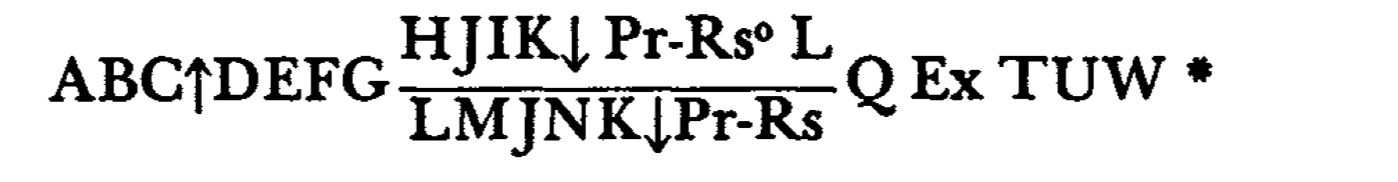
\includegraphics[scale=0.55]{figures/Propp.png}
    \caption{Propp's generalized fairytale with the set of functions ordered in a compositional scheme. Copied from \cite[105]{Propp1968}.}
    \label{fig:karstens:proppfairytale}
\end{figure}

In \figref{fig:karstens:proppfairytale} we see that a fairytale starts at A on the left and proceeds to G on the right. It can then either go up first, then down, and then proceed from Q to the end; or it can go up first and then directly to the end part; or down first then to the end part; or skip the middle part and move to the end part right away. Hence, not all functional elements have to be present in every story but, when they are, they always occur in the order given by the general type. It is also immaterial how and by whom the functions are performed. What matters is that these functions are performed in the story, and that this happens in a fixed order. Sequencing the functional elements is thus like establishing word order in a sentence and so it is possible to arrive at a grammar of stories. 

Propp created a new method of description, which he clearly hoped would raise the prestige of literary studies: ``What matters is not the amount of material, but the methods of investigation. At a time when the physical and mathematical sciences possess well-ordered classification, a unified terminology adopted by special conferences, and a methodology improved upon by the transmission from teachers to students, we have nothing comparable'' \citep[4]{Propp1968}. The morphological method of classification Propp introduced was inspired by the biological writings of Johann Wolfgang von Goethe (1749--1832). This involved the notion that we can identify fundamental ideas or archetypes (\emph{Urtypen}) underlying natural phenomena. The study of common patterns of development and modifications of the archetype was called ``morphology'' by Goethe.\footnote{According to \citet[257--258]{Steiner1984}, the return to Goethe was more widespread and stemmed from a growing dissatisfaction with positivism, which led scholars to explore scientific models that had existed before positivism became dominant. \citet[13]{Oppel1947} argues that the appearance of the Russian translation of Wilhelm Troll's (1897--1978) book \emph{Goethes morphologische Schriften} in 1926 paved the way for the acceptance of morphology as a respectable method. Alongside Propp, \citet{Petrovskij1927} also adopted the term. For the long-lasting influence of Goethe on the study of language and literature, see also \citet{Cassirer1945}.}

The generalized fairytale of \figref{fig:karstens:proppfairytale} can be considered the \emph{Urtyp} of all fairytales. Moreover, the word ``morphology'' in the title of Propp's book is a direct reference to Goethe; every chapter in the original publication is in fact preceded by an epigraph from Goethe's work. Following Goethe, Propp had an organicist understanding of functions: a function is an activity seen from the perspective of the relevance of this activity for the total course of action; that is, the story that is being told \citep[84]{Steiner1984}. With Propp, functions can never be studied in relation to an isolated task or goal. Each tale is thus perceived as a functionally integrated whole, and this distingishes him from members of the \textsc{opojaz} group, who saw works of art as mere aggregates of constituting elements.

Propp was very much focused on the description of the structure of the stories available in the present: ``We shall not speak at present about the historical study of the tale, but shall speak only about the description of it, for to discuss genetics, without special elucidation of the problem of description as it is usually treated, is completely useless. Before throwing light upon the question of the tale's origin, one must first answer the question as to what the tale itself represents'' \citep[5]{Propp1968}. But the analytical result that all folktales were basically of the same structure made Propp speculate about their origin. Could they all come from the same source? Moreover, he was well aware that \emph{Morphology of the Folk Tale} left open the crucial issue of how to get from the general type to the actual tales that occur in reality. What kind of transformations exist? And what explains their occurrence? 

Pressed by these issues, Propp devoted a separate essay to the subject, ``Fairy Tale Transformations'', which was first published separately and then as an appendix to the book (the original publication is \citealt{Propp1928}). He argued that synchronic comparative analysis and diachronic genealogical analysis could be undertaken separately, but in the end complemented each other. In the complementary paper, Propp discussed affinities that exist between the fairy tale and religion (myth and ritual) and various social institutions at different stages of their evolution. According to his analysis, the basic forms of fairy tales are religious. Changes into derived forms occur through ethnological and social processes. Hence, in order to understand the transformations (of which Propp specified 20 kinds) we must include external factors. But Propp did not make clear if a similar analysis can apply to all literary products. In his view, folk narratives were the products of collective creativity and came about through long-term social processes. They may thus differ in crucial respects from other literary works, such as novels and poems. The morphological approach was, however, tried on other literary genres as well, for example by Michael Petrovsky (1887--1940) and Aleksandr Skaftymov (1890--1968).  

\emph{Morphology of the Folktale} met with a late and peculiar reception in the West. Initially the work was not noticed internationally. This was probably an effect of the rise of Stalinism, which cut off intellectual exchange. The first translation into English, and to my knowledge into any Western language, appeared in 1958 with Indiana University Press.\footnote{Such delayed reception due to the political turmoil of the 1930s and 1940s occurred often. Emigrant scholars could make a ``second'' career in the United Kingdom or the United States. A well-known example is the sociologist Norbert Elias (1897--1990). In this context, it must be noted that the first translation of Propp's work into English is accompanied by an introduction written by Svatava Pirkova-Jakobson, the wife of Roman Jakobson.} This translation was however full of deficiencies. It also did not include the ``Fairy Tale Transformations'' appendix, and the Goethian epigraphs that preceded chapters in the original edition were conspicuously left out.\footnote{The 1968 second edition was of much better quality but still without the Goethian epigraphs, which were considered to be ``non-essential'' (preface by Louis A. Wagner).} 

Since structuralism was in full swing in 1958, the publication of \emph{Morphology of the Folktale} prompted a reaction from Lévi-Strauss in the form of a long review, which was published in French in 1960. Lévi-Strauss praised Propp for seeing through the rich semantic variety of fairy tales and for penetrating into the formal regularity of the stories. But he called it an error of formalism to disconnect syntax from the vocabulary (or lexicon). According to Lévi-Strauss, it is not possible to do formal analysis and content analysis separately: 

\begin{quotation}
For formalism, the two areas must be absolutely separate, as form alone is intelligible, and content is only a residual deprived of any significant value. For structuralism, this opposition does not exist; structuralism does not treat one as abstract and the other as concrete. Form and content are of the same nature, amenable to the same type of analysis. Content receives its reality from its structure, and what is called form is a way of organizing the local structures that make up this content. \citep[179]{Levi-Strauss1984}
\end{quotation}

As an illustration, he provided the example of bird names to stand for formal oppositions. According to Lévi-Strauss, the morphological approach cannot deal with the fact that the same bird names can be used to stand for multiple formal oppositions. This becomes especially problematic when in one case two bird names are in opposition, but in another case they together form one pole to oppose something else. As an example Lévi-Strauss gave ``day'' vs. ``night'', as expressed by an ``eagle'' vs. an ``owl'', and ``predators'' vs. ``scavengers'', which can be expressed by ``eagle + owl'' vs. ``crow'' or even ``sky-land'' vs. ``sky-water''; that is, ``eagle + owl + crow'' vs. ``duck''. Structural oppositions framed in this way involve the use of lexical meaning. For this reason, the formal opposition can only be understood when content is taken into account. In my view, the point Lévi-Strauss makes here resembles Mukarovsky's point that structuralism involves a synthesis between formal text analysis and meaningful interpretation through relating the text to the external context.

In addition to this, Lévi-Strauss also declared structuralism superior to formalism in that it did not have to stick to a linear basic structure but could shift from a syntagmatic (or temporal) order to a paradigmatic general structure. This paradigmatic structure is based on the recognition of a number of fundamental oppositional patterns and abstracts away from the temporal ordering of the story. In my view, the idea of making a distinction between a surface level and deeper levels of linguistic structure, with corresponding rules of transformation between them, is crucial to the structuralist approach to the study of language.\footnote{Deep structure, surface structure and transformation are of course Chomskyan terms, and used here somewhat anachronistically. But they are not far off the mark: according to \citet[1899--1900]{Joseph2001}, Chomsky's transformational grammar must be interpreted as a direct continuation of European structuralism (to contrast it with the significantly different American, Bloomfieldian structuralism which was challenged by Chomsky).} But even this does not yield a fundamental distinction between structuralism and formalism. Lévi-Strauss may have been correct in his assessment that organicist formalism lacked the means to abstract away from temporal order, but in the next section I will argue that the assumption of multiple levels of analysis in structuralism was inspired by another formalist variant, namely systemic formalism. 

Propp reacted to Lévi-Strauss' critical reception. This reaction was translated into Italian in 1966 and published together with an Italian version of \emph{Morphology of the Folk Tale}, accompanied by Lévi-Strauss' critical review of it. In his rebuttal Propp blamed the American translator:

\begin{quotation}
Professor Lévi-Strauss knows my book only in the English translation. But its translator allowed himself an impermissible liberty. Not understanding the function of the epigraphs which at first glance do not seem to be explicitly connected to the text, he considered them useless ornaments and barbarously omitted them […] all these epigraphs […] had the purpose of expressing what was left unsaid in the text of my book. (As translated in \citealt[81]{Steiner1984})
\end{quotation}

Propp also lamented that Lévi-Strauss had completely missed the importance of the plot for the understanding of a text as a functionally integrated whole. In this respect it is perhaps even more significant that the ``Fairy Tale Transformations'' complementary paper was not translated at all and only became available in English in 1971. The complementary paper demonstrates even more clearly that Propp had a profound interest in historical and ethnographic investigation and that he was willing to include ``content'' as an explanation for changes in the structure of fairy tales. It could even have become clear that Propp viewed this type of research as complementary to formalist analysis.

The aim of Propp's two-way publishing strategy was to optimize clarity of presentation, but the reception of Lévi-Strauss shows that this strategy may have had the opposite effect. Still, had the references to Goethe and ``Fairy Tale Transformations'' been known to Lévi-Strauss, I think that he would have maintained the two main points of his critique. For a structuralist to assume that formal and contextual analysis are complementary is insufficient; the two must be \emph{integrated}, since form and content simultaneously inform and determine each other. Mukarovsky charged mechanical formalism with neglect of external factors. While organic formalism in Propp's approach no longer did this, it still did not achieve the synthesis structuralists were seeking. Hence Lévi-Strauss could deliver a similar critique on Propp, even though the latter represented a different kind of formalism. Systemic formalism could, however, not be targeted in this way. This I will show in the next section.

\section{Systemic formalism and its points of contact with structuralism}
\label{sec:karstens:systemicformalism}

According to \citet[112]{Steiner1984}, systemic formalism represented the most advanced stage of the formalist movement. Significantly, it was called ``neo-formalism'' by contemporaries. Steiner connects the label systemic formalism for the most part to the work of Tynjanov, who put forward a dynamic, relationist understanding of literary structures. The literary theorist -- or, as the case may be, linguist -- had to account for the fact that linguistic structures are continuously unfolding, but at the same time that the recurrent systematic appearance of forms is what makes a language intelligible and understandable. In order to capture this double aspect of language, Tynjanov argued that a focus on experience alone is insufficient. Shklovsky counted as a formalist anyone whose analyses did not move beyond the sensory stratum, with a rather static theory as a result. According to Tynjanov, good science had to proceed both from taking direct experience into account \emph{and} from the assumption of a system, or deeper structure, that governs the way experiences come about. 

In this respect he was clearly inspired by Saussure's \emph{langue}-\emph{parole} distinction. The actual appearance of utterances (\emph{parole}) is a manifestation of the underlying linguistic system (\emph{langue}). For a number of reasons, Tynjanov very much liked the analogy between language and chess that Saussure had drawn. The positions we see on the chessboard depend on an unchangeable set of rules that exist before the game even begins. The analogy supports the relationist stance, because each piece receives its identity due to the system of rules \emph{and} its value is relative with respect to the other pieces on the board. The system of rules is strict, but it allows for a great degree of freedom of choice in the actual execution of moves. Finally, the social aspect of the analogy was attractive to Tynjanov: the system of rules has to be shared by players of the game, otherwise they cannot play. As written in chapter four of the \emph{Cours}, the socially shared linguistic code ``is necessary if speaking is to be intelligible and produce all its effects'' \citep[37]{Saussure19221916}. The analogy thus showed that both creative expression and human communication rest on a governing system.

Yet, as Steiner explains, there was a ``deep-seated difference'' between Saussure's and Tynjanov's thought about the autonomy of the \emph{langue} \citep[112]{Steiner1984}. While both wanted to establish an autonomous science of language (Saussure) and literature (Tynjanov, very much like \emph{all} the formalists), Saussure had insisted on absolute autonomy, but for Tynjanov autonomy was a relative notion. Tynjanov argued that any literary system was always part of an overall cultural system. This stance ``effected a gradual relativization of the original formalist position on the autonomy of the literary system'' \citep[111]{Steiner1984}. Where other formalists had made a sharp distinction between what was immanent to literature and what was not, Tynjanov started to blur this distinction and replaced it with a multi-layered conception of systems within systems.

A theory of relative autonomy was put forward in a 1928 paper co-written by Tynjanov and Jakobson titled ``Problems in the Study of Literature and Language'' \citep{Tyjanov1928}.\footnote{For the importance of this text in the genesis of structuralism, see \citet[17]{Holenstein1975}.} In this ground-breaking paper they presented nine theses on the historical development of language and literature and the relation between them. The eighth thesis reads:

\begin{quotation}
The discovery of the immanent laws of literature (language) permits us to characterize every concrete change in literary (linguistic) systems but does not permit us either to explain the tempo of evolution or to determine the actual selection among several theoretically possible evolutionary paths. This is because the immanent laws of literary (linguistic) evolution are indefinite equations which, while limiting the number of solutions, do not necessarily leave only a single one. Which pathway, or at least which dominant, is chosen can be determined only through an analysis of the correlation among the literary and other historical series. This correlation (the system of systems) has its own structural laws which should be studied. \citep[Quotation given in English in][128]{Steiner1984}
\end{quotation}

Tynjanov and Jakobson saw the entire culture as a complex system of systems. Each subsystem has its own immanent set of rules but is also determined by the larger system of which it is part, which can lead to a change in rules in the subsystem itself.

The authors perceived a deep relation between language and literature, and hence also between the science of language and the science of literature. These two formed more than just a continuum: both disciplines had to be based on the same principles. The literary genre of poetry provides a good illustration of this commutativity \citep[see][]{Jakobson1981poetry,Jakobson1981landp}. Poetry is made of language; therefore linguistics directly informs the writing of poems. But structuralists also investigated poetry as a special function of language. Because in poetry it is possible to break the natural ties between signifier and signified, it is also possible to experiment in poetry and self-reflexively develop the language that is being used.\footnote{On the redefinition of the notion of function in semiotic terms and the use of functions in Jakobson's structuralism, see the next section.} The 1928 paper established a connection between formalism, which pertained to literary studies, and structuralism, which mostly pertained to linguistics. From this it becomes understandable that Jakobson, the linguist, and Mukarovsky, the literary scholar, could collaborate in the development of structuralism in the context of the Prague Linguistic Circle. 

Systemic formalism differed from mechanical formalism in that it no longer searched for an unchanging literary essence. It also did not explain the history of literature as an immanent process. Systemic formalists analyzed both the structural relations within a single literary product \emph{and} the relations of this work with the rest of literature and with the whole culture of the time in which the work was written and published. All of these realms were conceived as systems containing sets of interdependent variables. In this way, a literary work was itself seen as a variable in a system of higher order.  

The difference between organic formalism and systemic formalism was subtler, yet very significant. Like the systemic approach, the morphological approach was also anti-positivistic and had a functional understanding of the role elements play in relation to the purpose (artistic goal) of the whole. The whole is a system because of the interplay of functional elements that work together to achieve the common goal. But in systemic formalism the notions of system and function got a different definition. A function in systemic formalism is seen as a relation of two interdependent variables and a system was conceived as a hierarchical set of interdependent variables. To call literature a system in this sense was extremism or radicalism to adherents of the morphological approach.

In my view, a highly important difference is at stake here. In historiography of linguistic structuralism, we often confront the ``standard'' interpretation that the organic way of thinking of 19th century historical and comparative linguistics, with August Schleicher's (1821--1868) morphology perhaps as the most distinctive representative, paved the way for the systematic/structural way of thinking of the 20th century.\footnote{A clear example of this interpretation, which even reached the major handbook of the history of the language sciences, is \citet{Kohrt2001}.} To conceive of languages as structures is then simply the continuation of the application of the organism metaphor; that is, to conceive of a language as a living organism. What matters in both structuralist and comparative linguistics is to unravel the (reciprocal) relations between parts and the whole of the linguistic structure/organism. Fitting to this account would be a reference to organic formalism as a source of inspiration for linguistic structuralism. But, as we have seen above, it is systemic formalism that mostly influenced linguistic structuralism and not the morphological approach. In my view, it follows that the ``standard'' continuity interpretation must be seriously questioned. 

Notwithstanding the similarity between organic formalism and structuralism with respect to holistic analysis, the morphological approach does not dig to a deep level of systematic analysis. It remains quite closely tied to the empirical ``sensory stratum''; if we were to think, for example, of the skeleton as a structure of bones. In this sense it was still relatively close to mechanic formalism. Systemic formalism, on the other hand, involved a fundamental shift in thinking. The approach rested on the recognition of multiple systems, hierarchically ordered in levels. This conception did not only apply to a view of the system of language within broader cultural systems, but also to the study of language itself. I believe this helped to pave the way for the distinction structuralists made between a surface, or manifest, level of actual occurring written or spoken speech, and a deeper level of structural relations that underlie occurrences at the manifest level.

This of course had to be accompanied by a theory of the transformations from one level to another. Such theories became customary in postwar linguistics, even if not always under the banner of structuralism, and sometimes even opposed to it. Given this long-lasting impact, the final section of paper explores how the ideas of systemic formalism were incorporated as elements of a larger merger of constituents of structuralism.

\section{Structuralism as a merger of multiple constituents}
\label{sec:karstens:structuralism}

The historiography of structuralism has been dominated by the so-called ``French model'' \citep[cf.][]{Flack2016}. In this model, structuralism starts with the Swiss, but French-speaking, Saussure and after a brief intermediary phase is further developed by Lévi-Strauss and via him disseminated in many fields of study. I agree with two recent papers that this model is at best incomplete and should be replaced by a model that involves a much wider circulation perspective \emph{and} that makes the figure of Roman Jakobson occupy centre stage \citep[see][]{Percival2011,Flack2016}. This central position is justified because Jakobson was part of both the Moscow formalism and futurism of the 1910s and the Prague Circle in the 1920s and 1930s. He was the first to use the very term structuralism in linguistics and contributed significantly to developing it, in the early years first and foremost in the area of phonology. Due to his exile in the United States, he directly influenced Lévi-Strauss, who was also exiled for a while in New York, and after the war his thought had an impact on important linguists such as Morris Halle (1923--2018) and Noam Chomsky (b. 1928). 

The study of the circulation of knowledge should investigate the crossing of temporal, geographical as well as disciplinary boundaries. The latter is especially relevant when it comes to providing an account of the genesis of structuralism. Jakobson was an extremely versatile scholar who fused together constituents of structuralism from a variety of sources.\footnote{``Das Werk [of Jakobson, like that of Leibniz] ist gekennzeichnet durch eine breitgefächerte Forschungstätigkeit, die ans Unglaubliche grenzt'' \citep[17]{Holenstein1975}. In \citet{Karstens2017lonely}, I argue that the pursuit of a number of key virtues helped Jakobson to fuse together a variety of elements to a more or less coherent approach to the study of language. In this respect, see also \citet{Karstens2017blog}.} Among these are the concepts of \emph{Gestalt} from psychology, ``invariance'' from mathematics, ``limited variation'' from biology, ``periodicity'' from chemistry, and from phenomenology the central role of ``expression'', the importance of the notion of ``opposition'' and the anti-positivist stance.\footnote{For the influence of phenomenology on structuralism, the main point of reference has for quite some time been \citet{Holenstein1975}, but also see \citet{Flack2016}.} Members of the Prague School were therefore not as hostile to philosophical ``speculation'' as the Russian formalists had been, as they aligned their core anti-positivist stance to phenomenology and to the philosophically informed Gestalt psychology.\footnote{The widespread anti-psychologism of the time did not involve a complete rejection of psychology, but a rejection of ``bad'' psychology and of an ill-founded connection between linguistics and psychology that members of the Prague circle, for example, found in the work of Wilhelm Wundt (1832--1920). See \citet[139]{Toman1995}.} However, as in formalism, we find the inclusion of ideas from the natural sciences, which the practitioners of structuralism could use to claim a respectable place in the disciplinary landscape. But, significantly, Jakobson, took this alliance a step further. The very first time he mentioned the term structuralism he did not connect it to linguistics only, but immediately raised it to the status of a \emph{science générale}:

\begin{quotation}
Were we to comprise the leading idea of present-day science in its most various manifestations, we could hardly find a more appropriate designation than structuralism. Any set of phenomena examined by contemporary science is treated not as a mechanical agglomeration but as a structural whole, and the basic task is to reveal the inner, whether static or developmental, laws of this system. What appears to be the focus of scientific preoccupations is no longer the outer stimulus, but the internal premises of development; now the mechanical conception of processes yields to the question of their functions. \citep[11]{Jakobson1929}
\end{quotation}

Two things are striking in this citation. The first of these is the distinction that is drawn between two levels, namely ``the outer stimulus'' and an inner system, seen as a structural whole. The second is the importance that Jakobson attached to the investigation of functions of this structural whole. As was discussed above, both the concepts of system and function played a central role in systemic formalism. Here I want to investigate how to place these concepts in the broader amalgam of structuralism.

An important idea that structuralists took over from systemic formalism is that, in order to be intelligible, language has to have recurrent properties. That is, the regular appearance of linguistic forms is what makes language understandable and hence apt as a medium of communication. Russian futurists had made a similar point in their call for cultural \emph{and} linguistic reform in the 1910s and 1920s.\footnote{There were many connections between futurism and formalism; this is one of the main themes of \citet{Toman1995}.} Their approach must be contrasted with Italian futurism. The difference became apparent when Filippo Marinetti (1876--1944), the author of the ``Manifesto del Futurismo'' (\citeyear{Marinetti1909}), paid a visit to Moscow in 1914.\footnote{Interestingly, the young Jakobson acted as an interpreter at this event. See \citet[17]{Toman1995}.} In a lecture he gave there, Marinetti proposed to liberate speech by freeing words from the bonds of grammatical rules and by using onomatopoetic and emotive interjections to create expressions that appeal directly to the senses \citep[87--88]{Gasparov2014}.\footnote{Such ideas about language reform were not uncommon at the time. Both in Dada and other surrealist movements, spontaneous language use, freed from rules and ``formulas'', was promoted. See, for example, \citet{Spaendonck1977}.} The Russians found this approach extremely shallow. They argued that meaningful variation is only possible given the structure of a language and the existing tradition of language use in a community of speakers. Successful reform could only be achieved by gaining a deeper understanding of the systematic aspects of the language and by effecting meaningful and lasting reform from such knowledge. Hence the advancement of the investigation of a deeper-level system behind surface-level occurrences of linguistic expressions. 

The Russian avant-garde explored relations between constituents of music, painting and poetry. They wanted to know which constituents were basic or ``invariant'', and explored the limits set on combinations of consituents. Their goal was to create a basis for free creativity, without any utilitarian purpose. It was generally thought that elementary forms that appealed to everyone would provide such a basis \citep[238--239]{Toman1995}. When Jakobson said, ``we learned from the poets'', he was referring in particular to Khlebnikov, the futurist poet who was influential in the Moscow Linguistic Circle, the Moscow counterpart of the Petersburg \textsc{opojaz} group \citep[see][]{Jakobson1979}.\footnote{ \citet[10--11]{Toman1995} mentions an early interest by Jakobson in the formal aspects of folkore, Russian dialects and poetry. One of the first major papers he wrote was an essay on Khlebnikov.} Khlebnikov thought that knowledge of basic structural relations could show unused realms for the expressions of meaning and help to determine the scope of meaningful variation. But this knowledge still had to be won. He drew inspiration from chemistry in this respect: ``The entire language is to be divided into its fundamental elementary truths, whereafter it would be possible to build for sounds something similar to Mendeleev's law, that last pinnacle of chemical thought'' \citep[Khlebnikov as translated in][95]{Gasparov2014}. This ``law'' states that chemical and physical properties of the elements recur periodically. By analogy, Khlebnikov expected that periodicity could also be found when the basic elements of language were arranged in systematic order. 

Jakobson and his fellow structuralists took up Khlebnikov's challenge. Since phonemes are the smallest units of sound capable of distinguishing units of meaning in language, a basic set of phonemes could be the basic elements of language that Khlebnikov was looking for.\footnote{In fact, the great breakthrough was to go one layer deeper and consider phonemes as bundles of constitutive features. These features then are the real basic elements of language.} It is therefore not a coincidence that Prague structuralists focused on phonology, the area that studies the systematic organization of sounds in languages; that is, the system of phonemes. Phonology was simply seen as the most basic science of language. Jakobson's research yielded an integral system of sets of minimal oppositions between the phonemes of a language. The system of minimal pairs set limits on the possible sound combinations out of which words can be created and which eventually occur on the surface level in language use. 

We can therefore see how ideas about systematic organization from formalism connected to Russian futurism and found their way into structuralist phonology. The mathematical concept of ``invariance'' and the somewhat offbeat biological concept of ``limited variation'' fitted in here too. The concept of invariance allowed structuralists to express linguistic relations in mathematical terms. In Leo Berg's (1876--1950) evolutionary theory limits are set on variation, as variation was thought to be strongly contained by morphological forms. This theory thus differs from Charles Darwin's (1809--1882) idea of random variation and selection through environmental pressures. Jakobson was attracted to Berg's theory because it corresponded to limits set on word formation through a system of basic forms of language.

The idea of distinguishing between a surface level and a deeper system was most probably drawn directly from the work of Saussure.\footnote{\citet[88--94]{Toman1995} mentions that Jakobson ordered a number of French books in 1921 when he was studying in Prague which included the \emph{Cours}. Also his first investigations into phonological systems were accompanied by references to Albert Sechehaye (1870--1946).} According to \citet[237]{Joseph2010}, Saussure achieved the conceptual leap to consider phonemes not as sound as such, but as units within a system: ``Saussure's impact on 20th century linguistics would include the simplification brought about by the reorientation away from sound as such, and toward systems and the units that compose them. This would be the basis for the movement known as structuralism.” It is not entirely clear where the conceptual leap of Saussure came from. Some have suggested that he was inspired by an analogy with economics, others see an impact of the periodic system of Mendeleev (1834--1907) on Saussure too.\footnote{The economic theory is discussed in \citet{Joseph2014}. For the chemistry case, see \citet{Culler1976}, \citet{Clark2008} and \citet{Silverstein2016}.} But in the absence of concrete references the case is hard to make. 

The distinction between surface structures and a deeper governing system Jakobson most likely took over from Tynjanov's systemic formalism, Khlebnikov's futurism \emph{and} directly from Saussure. Moreover, Jakobson liked to draw analogies between linguistic structures and biological or physical structures which included those found in geology (earth layers) or meteorology (isolines) \citep[see][74--74, 188--194]{Holenstein1975}. For him all these links could only confirm the hypothesis that structuralism was the appropriate designation for science ``in its most various manifestations''.\footnote{A position that was fully vindicated through Cassirer's wide-ranging philosophical discussion of structuralism in \citet{Cassirer1945}.}  

Likewise, the concept of function could be applied in more than one scientific discipline. Turning to Prague structuralism, \citet{Steiner1976} has argued that the three basic theoretical concepts -- structure, function and sign -- were complementary notions interwoven into a cohesive approach. This is because structures have to be differentiated according to their dominant functions, and the semiotic function has the capacity to turn every object it dominates into a sign. Elsewhere Steiner explains how the formalist primary concept of function was redefined in semiotic terms \citep[264--266]{Steiner1984}. He argues that structuralists needed the notion of function because they considered all of reality, from sensory perception to the most abstract mental construction, as a vast and complex realm of signs. There was therefore a need for some criterion to differentiate individual semiotic structures from each other. In structuralism the guiding thought is that every element in language exists because it has a function to fulfil. A function is defined as an active relation between an object and the goal for which the object is used.\footnote{Note that this teleology is anathema to a mechanistic worldview.} In this way we can distinguish between the communicative, practical (or social) function of language and poetic, or artistic/aesthetic function. Function in this sense thus does not apply to the function of an element in a literary text, but rather to the dominant function of a particular semiotic structure. On my estimation, this does not exclude functional interpretation in the former sense. The semiotic understanding of functions just adds another dimension to the application of the function concept of systemic formalism.

Structuralism, like formalism and Saussure before, aimed to establish an independent science of language. The claim for independence prompted an alignment with models and theories stemming from a great variety of directions, including the natural sciences. I hope to have shown that systemic formalism provided a number of key elements of structuralism. If these elements partially overlapped with other sources of inspiration, this would only provide an extra assurance that they were rightly elected as being part of the structuralist programme. 

\section{Conclusion}
\label{sec:karstens:conclusion}

\citet{Steiner1984} wittily presents the formalist movement as a \emph{polemos}. Formalists shared the common goal of changing the scholarly practice of literary studies and establishing a new autonomous realm for the discipline, but disagreed about how to achieve that goal. The formalists themselves were each other's fiercest critics. Boris Ejchenbaum (1886--1959) embraced this state of affairs in 1922, exclaiming: ``Enough of monism! We are pluralists. Life is diverse and cannot be reduced to a single principle'' \citep[quoted in English in][259]{Steiner1984}.

In general, three main types of formalism can be distinguished. Two of these, mechanical and organic formalism, differed at crucial points from structuralism but with a third variation, systemic formalism, such a clear distinction cannot be drawn. In structuralism we can therefore find a number of key aspects of systemic formalism, such as the application of the notion of function, the importance of the systematic recurrence of forms in language, the idea of analysing manifestations of language use with reference to a deeper system, and placing the linguistic system within broader social and cultural systems; that is, thinking in terms of systems within systems. These points of continuity came about in part through a direct collaboration between Tynjanov, the leading systemic formalist and Jakobson, the leading linguistic structuralist.

Systemic formalism was constitutive of the new direction in which general linguistics headed, as it helped to define object, aim and task of linguistic study. In structuralism, formalist ideas merged with constituents stemming from other directions, including phenomenology, biology, mathematics and Saussurian linguistics. Mukarovsky tended to consider structuralism as an attitude instead of a distinct linguistic theory. This attitude was synthetic rather than pluralistic. Structuralists wanted to overcome oppositions between form and content, data and interpretation, synchrony and diachrony, \emph{langue} and \emph{parole}, etc. It was therefore natural to combine ideas from all kinds of directions to achieve the sought-after synthesis.\footnote{\citet[150--152]{Toman1995} includes a section on the ``Courage to synthesize''. He firmly places the synthetic attitude in the context of dialectics but this is perhaps unnecessary. A synthetic attitude may just involve fusing things together from different directions.} We find this attitude most clearly in Roman Jakobson, who was an extremely versatile scholar and who was instrumental in carrying structuralist ideas to the Western world. I agree with \citet{Steiner1984} that Russian formalism is best considered a transitory phase in the history of literary studies and linguistics. While the formalist programme as a whole came to an end, components of it did not, and this was in no small part due to the rise of structuralism as a major approach in linguistics. 

\section*{Acknowledgements}

I would like thank my colleagues Emma Mojet and Sjang ten Hagen for their careful reading of a draft version of this paper.

\sloppy
\printbibliography[heading=subbibliography,notkeyword=this] 
\end{document}